


\section {Motivation}

Newspapers are rich sources of history and millions of pages of historical newspapers have been digitized \cite{Allen_10} in recent years. A national program to develop an Internet-based, searchable database of U.S. newspapers called the National Digital Newspaper Program (NDNP) was setup in 2004 as a partnership between the National Endowment of Humanities (NEH) and the Library of Congress. Since then, several public and for-profit sectors have also digitized newspapers at a rapid pace making text from historical records available at a staggering rate. To deal with this wealth of information, scholars have mainly focused on text mining and information retrieval techniques followed by visualization of patterns extracted from the records \cite{McKeown_1995, Radev99c, mckeown2002tracking, dutta2011learning, Berberich_2007, khurdiya2011multi, shahaf2010connecting}. 


\begin{figure*}[t]
\begin{center}
%\mbox{
\subfigure[GenealogyBank]
{
%%\includegraphics[width=0.6\columnwidth]{odds_20070813_160000rb_M.pdf}
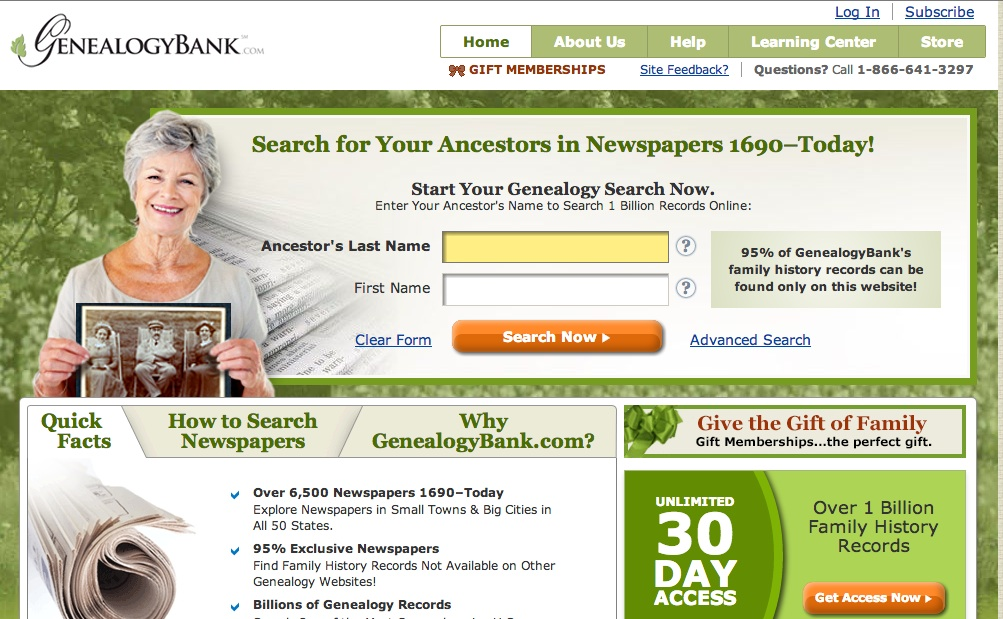
\includegraphics[width=0.43\textwidth, height=0.23\textheight]{genealogy.jpg}
\label{fig:gen}
}
\subfigure[FamilySearch]
{
%%\includegraphics[width=0.8\columnwidth]{20070813-C1-7d-roc.pdf}
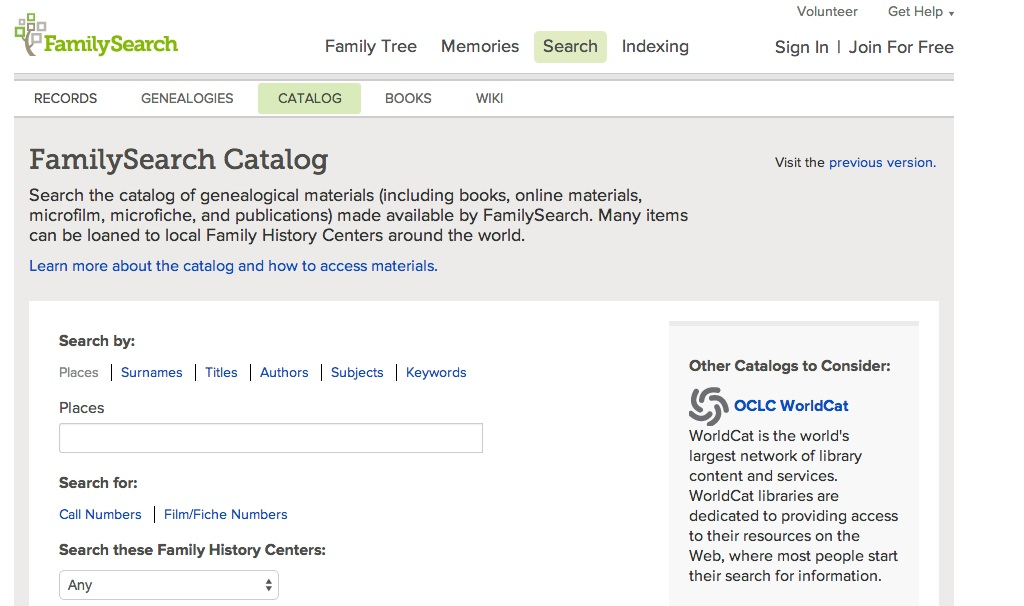
\includegraphics[width=0.43\textwidth, height=0.23\textheight]{FamilySearch}
\label{fig:fam}
}
%}
\caption{Two examples of online People Search Tools which utilize historic newspaper archives, military records, petitions, obituaries, census records and other forms of petitions to match proper nouns.}
\label{figSearch}
\end{center}
\end{figure*}

An important use of historical newspapers is for People Search\cite{BilenkoMCRF03,Friedman_92}) -- for example, to find important people and track the timelines of news articles related to them. Several websites like Genealogy Bank\footnote{http://www.genealogybank.com/gbnk/}, FamilySearch\footnote{https://familysearch.org/}, Newspaper Archives\footnote{http://newspaperarchive.com/}, Ancestry\footnote{http://www.ancestry.com/} provide people search service that include obituaries, birth and death lists, newspaper articles, military records, Revolutionary and Civil War pension requests, census records, land grants and other forms of petitions. Figure~\ref{figSearch} shows two such tools available online.

%Existing literature also deals with the problem of spelling variations in people names -- solutions include use of Soundex\footnote{http://www.myheritage.com/FP/Company/megadex.php} technology that given a query, returns everything that ``sounds like" what the query term. Face recognition algorithms, video and audio clips have been used to enhance search. However research in this domain is still in its nascent stages.


%Information related to a person can be extracted from online freely available historical archives of newspapers for which the text requires cleaning and preprocessing to make the information available in the required format.
  
To the best of our knowledge, the problem of finding \emph{influential} people from historic newspaper archives has not been studied before. This exercise, however, opens up a wide range of possibilities -- for example, news articles related to the influential person can also be linked to a Wikipedia page entry to find out relevant details or build influential people networks that can learn about entities involved in historical events. 

\section{Problem Description}
\label{problem}
%%DOUBT: DIFFERENCE BETWEEN AIM AND PROBLEM DESCRIPTION? DO THEY NEED TO BE MENTIONED SEPARATELY?


The goal of this research is to find and rank influential people across multiple topic categories in historical newspaper OCR archives.


%DOUBT:  IS IT OK TO MENTION THESE DETAILS HERE OR THEY SHOULD BE WRITTEN IN RELATED WORK?
%The problem of finding influential people in this scenario is a novel one as much of the research work deals with identification of influential nodes in social networks or marketing and diffusion research. This research does not involve finding influential people in terms of their influence on their peers\cite{watts2007influentials} or influence propagation in a social network \cite{kempe2003maximizing} which is how the concept of influence is used in general.   

 An influential person can be defined as ``a person whose actions and opinions strongly influence a course of events". This allows us to link an influential person with a list of articles that s/he occurs in.
 A person may also be considered influential if s/he gets talked about frequently in news articles. The problem can be also be phrased as identifying and ranking \emph{popular} people across various categories in the news domain. 
 ``Popularity" has been defined in other domains by counting number of votes, tweets, citations and followers. \cite{cheng2014can} but similar measures are not applicable in a newspaper setting where only the newspaper articles mentioning multiple people names are available.  
 
We divide the the problem of finding influential people into the following subproblems:
\begin{itemize}
\item \textbf{Problem 1: } Spell Correction and Cleaning of OCR text
\item \textbf{Problem 2: } Development of a People Gazetteer -- develop an organized structure in order to ease the process of identification of influential people.
\item \textbf{Problem 3: } Influential People Identification -- define the criteria for identifying and ranking people as ``influential".
\end{itemize}
  
%Each of the above problems require consideration of the dataset size and characteristics along with the newspaper environment in mind. 
\begin{figure}[h]
\centering
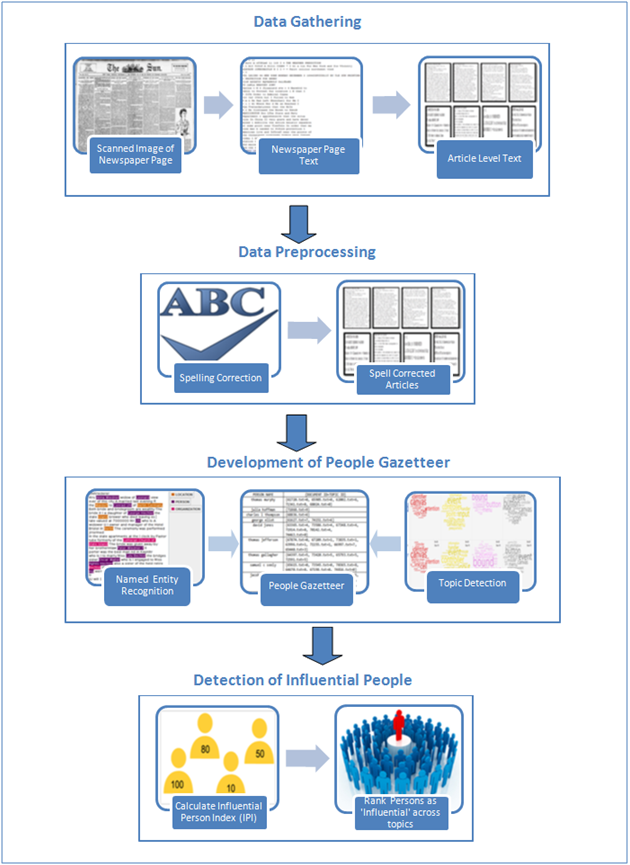
\includegraphics[width=0.6\textwidth, height=0.5\textheight]{framework3}
\caption{Research Framework showing components of proposed solution}
\label{fig:framework}
\end{figure} 

\section {Research Framework}

We propose the following solution framework in Figure~\ref{fig:framework} for finding influential people from a historical news repository. Each component is briefly described as follows:

\begin{enumerate}
\item \textbf {Data Gathering}:  
This component describes the source of data along with relevant statistics. It also includes descriptions of how the page level newspaper images are converted to text through OCR followed by article level segmentation. The different types of OCR errors encountered in the data are also described. This component is further discussed in Chapter ~\ref{chapter:data description}.

\item \textbf {Data Preprocessing}:
This component describes the preprocessing applied on the news articles. It describes relevant spelling correction algorithms, and then presents a novel algorithm for evaluation of the results. This component is further discussed in detail in Chapter ~\ref{chapter:data preprocessing}.

\item \textbf {Development of People Gazetteer}:
This component describes the process of development of people gazetteer which involves Named Entity Recognition in order to find person entities. This is followed by topic detection using LDA to assign topics to news articles and link both to obtain an organized structure. This component is discussed in detail in Chapter ~\ref{chapter:people gazetteer}.

\item \textbf {Influential Person Identification}:
This component defines an ``Influential Person Index" (IPI) that incorporates several criteria for identifying and ranking of ``influential people" across newspaper topics. Details about IPI, ranking and final results with some case studies are discussed in Chapter ~\ref{chapter:influential people detection}.

\end{enumerate}
 


%DOUBT: EITHER WRITE AS WE AIM TO ANSWER THESE QUESTIONS IN THIS RESEARCH OR WE DIVIDE THE PROBLEM INTO THESE SUBPROBLEMS...
%We aim to answer the following questions related to the problem of finding influential people with this research:
%Question 1 : How to deal with OCR data consisting of extremely noisy text for such a task?
%Question 2 : How to develop and use an organized structure for easy identification of influential people?
%Question 3 : Who are `influential persons" in a newspaper scenario and how to rank them?


%DOUBT: NOT SURE WHETHER RESEARCH FRAMEWORK SHOULD COME FIRST OR NOVEL CONTRIBUTION?
\section{Research Contributions}
\label{intro:rc}
This thesis has the following novel contributions:
\begin{enumerate}
\item A new algorithm for \emph{evaluation} of the performance of the spelling correction algorithm is presented. 
\item Development of the People Gazetteer -- an organized dictionary of people names and a list of articles in which the name occurs along with the corresponding topic of each article to facilitate identification of influential people.
\item Define an Influential Person Index (IPI) and metrics for its calculation in order to identify and rank influential people. Case studies of the top-K influential people detected are also discussed and verified with Wikipedia data. 

\end{enumerate}


